% CCAI Summer School 2026 — AI for Forestry
% Companion slide deck for the tutorial
%   "Detecting Deforestation from Satellite Image Time Series"
% Compile:  pdflatex deforestation_sits.tex   (run twice for the ToC/progress bar)
\documentclass[aspectratio=169,11pt]{beamer}

\usetheme{metropolis}
\usepackage{appendixnumberbeamer}
\usepackage{booktabs}
\usepackage{graphicx}
\usepackage{amsmath}
\usepackage{xcolor}
\usepackage{tikz}

\graphicspath{{../figures/}}

% --- palette matching the tutorial figures -------------------------------
\definecolor{forestgreen}{HTML}{008300}
\definecolor{accentblue}{HTML}{2A78D6}
\definecolor{clearred}{HTML}{E34948}
\definecolor{pastureyellow}{HTML}{C98500}
\definecolor{inkgrey}{HTML}{52514E}

\setbeamercolor{frametitle}{bg=forestgreen}
\setbeamercolor{progress bar}{fg=accentblue}
\setbeamercolor{title separator}{fg=accentblue}
\setbeamercolor{alerted text}{fg=clearred}

\metroset{sectionpage=progressbar, numbering=fraction, progressbar=frametitle}

% compact helper for source lines
\newcommand{\src}[1]{{\scriptsize\color{inkgrey}#1}}
\newcommand{\gtag}[1]{{\color{forestgreen}\textbf{#1}}}

\title{Detecting Deforestation from Satellite Image Time Series}
\subtitle{From a 1D-CNN to a Transformer and AlphaEarth embeddings \textbullet\ CCAI Virtual Summer School 2026}
\author{AI for Forestry tutorial}
\date{}

\begin{document}

{\setbeamercolor{background canvas}{bg=white}
\maketitle}

% =========================================================================
\begin{frame}{What this deck covers}
  \tableofcontents
\end{frame}

% =========================================================================
\section{Why this problem matters}

\begin{frame}{The climate case for watching forests}
  \begin{columns}[T]
    \begin{column}{0.58\textwidth}
      \begin{itemize}
        \item Tropical deforestation is one of the largest sources of
              greenhouse-gas emissions \alert{after fossil fuels}.
        \item A standing forest \emph{absorbs} carbon; a cleared-and-burned
              forest \emph{releases} it.
        \item \textbf{$>$420 million ha} of forest lost 1990–2020, $>$90\% in
              the tropics \src{(IPCC AR6, Ometto et al. 2022)}.
      \end{itemize}
      \vspace{0.4em}
      \begin{alertblock}{The first step is measurement}
        You cannot manage what you cannot measure. Reliable, \emph{timely} maps
        of \emph{where} and \emph{when} clearing happens are the foundation.
      \end{alertblock}
    \end{column}
    \begin{column}{0.42\textwidth}
      \small
      \textbf{Who acts on these maps}
      \begin{itemize}
        \item \textbf{Policy} — Brazil's PPCDAm helped cut Amazon loss
              $\sim$80\% (2004–2012).
        \item \textbf{Enforcement} — INPE's DETER daily alerts direct IBAMA
              field inspections.
        \item \textbf{Trade} — EU Deforestation Regulation (EUDR 2023/1115)
              bans commodities on land cleared after Dec 2020.
      \end{itemize}
    \end{column}
  \end{columns}
\end{frame}

\begin{frame}{The task, in one sentence}
  \begin{block}{Problem framing}
    Treat every location on the ground as a \gtag{time series} of a greenness
    index across one year, and \gtag{classify} each series as
    \emph{stable forest}, \emph{deforested this year}, or \emph{old clearing}.
  \end{block}
  \begin{itemize}
    \item Forest that is cleared shows a characteristic \alert{drop}; forest
          left intact does not.
    \item This is the same \emph{Satellite Image Time Series} (SITS) framing
          INPE uses in its \texttt{sits} / Brazil Data Cube pipeline.
    \item \textbf{Learning goals:} understand SITS, build \& compare a baseline
          and a deep model, read the evaluation honestly, and reason about
          responsible use.
  \end{itemize}
\end{frame}

% =========================================================================
\section{Key concepts}

\begin{frame}{Concept 1 — NDVI, a ``greenness'' number}
  \begin{columns}[T]
    \begin{column}{0.55\textwidth}
      Healthy vegetation reflects lots of \textbf{near-infrared (NIR)} light and
      absorbs \textbf{red} light. NDVI combines the two bands into one value in
      $[-1, 1]$:
      \[
        \mathrm{NDVI} = \frac{\mathrm{NIR} - \mathrm{Red}}{\mathrm{NIR} + \mathrm{Red}}
      \]
      \begin{itemize}
        \item Dense forest: \gtag{0.8–0.9}
        \item Pasture / bare soil: \alert{much lower}
      \end{itemize}
    \end{column}
    \begin{column}{0.45\textwidth}
      \begin{exampleblock}{Why one index?}
        NDVI compresses a multi-band image into a single, interpretable number
        per pixel — small enough to teach with, and directly tied to how much
        living vegetation is present.
      \end{exampleblock}
      \src{We derive NDVI from Sentinel-2 bands B04 (red) and B08 (NIR).}
    \end{column}
  \end{columns}
\end{frame}

\begin{frame}{Concept 2 — Why a \emph{time series} beats a single image}
  \begin{columns}[T]
    \begin{column}{0.5\textwidth}
      \begin{itemize}
        \item A single tropical image is often \alert{useless} — clouds, haze,
              shadow.
        \item A single \emph{date} also can't tell ``low today'' from
              ``dropped this year''.
        \item The \gtag{shape over time} — a mid-year fall from high to low —
              is the signal that identifies a clearing event.
      \end{itemize}
    \end{column}
    \begin{column}{0.5\textwidth}
      \centering
      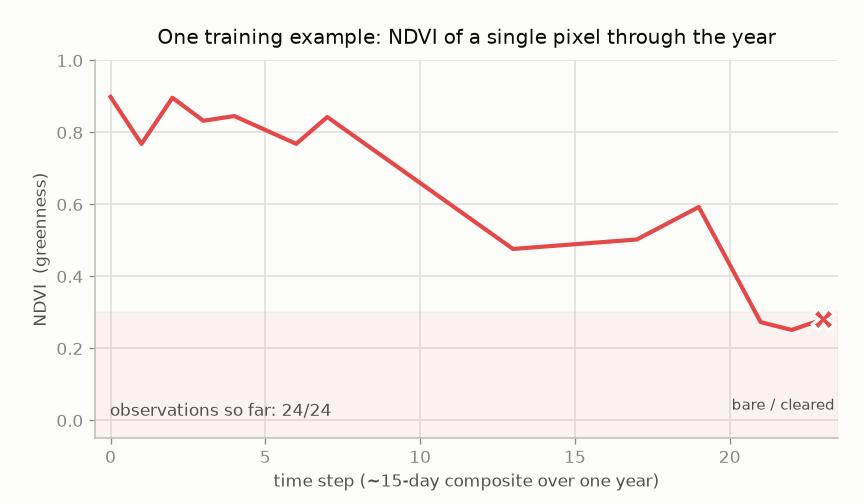
\includegraphics[width=\linewidth]{fig_01b_example.png}\\
      \src{One pixel's NDVI across a year: high, then a drop as it is cleared.}
    \end{column}
  \end{columns}
\end{frame}

% =========================================================================
\section{The study area \& the data}

\begin{frame}{Study area — an active frontier in southern Pará, Brazil}
  \begin{columns}[T]
    \begin{column}{0.55\textwidth}
      \begin{itemize}
        \item Bounding box \texttt{[-54.75, -3.70, -54.55, -3.50]} — a
              $\sim$22$\times$22 km window on the BR-163 / Rio Novo arc.
        \item Chosen because it contains \gtag{both} intact forest and
              multi-year PRODES clearings, and stays small enough to rebuild
              quickly.
        \item Season: \textbf{Aug 2021 – Jul 2022}, matching the PRODES 2022
              reporting year.
      \end{itemize}
      \begin{alertblock}{One region, one year, one sensor}
        Deliberately narrow for teaching — and the reason results here
        \emph{do not generalise} (revisited under Limitations).
      \end{alertblock}
    \end{column}
    \begin{column}{0.45\textwidth}
      \centering
      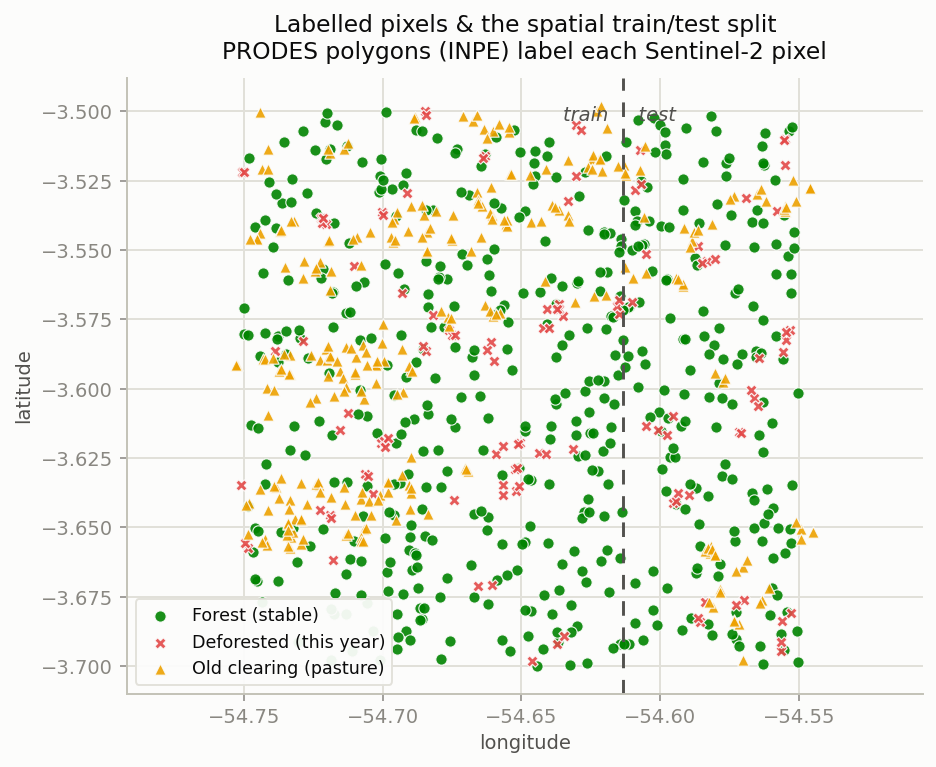
\includegraphics[width=\linewidth]{fig_02_labels.png}\\
      \src{Every dot is a labelled pixel; colour = class.}
    \end{column}
  \end{columns}
\end{frame}

\begin{frame}{Data source 1 — the imagery: Sentinel-2}
  \begin{columns}[T]
    \begin{column}{0.6\textwidth}
      \begin{itemize}
        \item \textbf{Sentinel-2 L2A} surface reflectance (ESA Copernicus),
              free and open, $\sim$5-day revisit.
        \item Bands used: \textbf{B04 (red)}, \textbf{B08 (NIR)} for NDVI, plus
              the \textbf{Scene Classification Layer (SCL)} for cloud masking.
        \item Resampled to a \gtag{20 m} pixel grid.
        \item Accessed programmatically via the \textbf{Microsoft Planetary
              Computer} STAC API — no bulk downloads.
      \end{itemize}
    \end{column}
    \begin{column}{0.4\textwidth}
      \begin{exampleblock}{Real-world condition}
        106 Sentinel-2 scenes intersect our window in one year, but the wet
        season (Dec–Mar) is \alert{heavily clouded} — a core difficulty, not an
        edge case.
      \end{exampleblock}
    \end{column}
  \end{columns}
\end{frame}

\begin{frame}{Data source 2 — the labels: INPE PRODES}
  \begin{columns}[T]
    \begin{column}{0.6\textwidth}
      \begin{itemize}
        \item \textbf{PRODES} is INPE's official annual clear-cut deforestation
              map for the Amazon — the reference standard for Brazil.
        \item We pull two layers from the open \textbf{TerraBrasilis} WFS:
              \begin{itemize}
                \item \texttt{yearly\_deforestation} — clearings by year
                \item \texttt{accumulated\_deforestation\_2007} — everything
                      cleared before
              \end{itemize}
        \item Polygons are expert-reviewed, with a \gtag{1-ha} minimum mapping
              unit and an annual cadence.
      \end{itemize}
    \end{column}
    \begin{column}{0.4\textwidth}
      \begin{alertblock}{Labels have limits too}
        Annual (not instant), clear-cut focused — \emph{degradation} and
        selective logging are only partly captured. Our labels inherit these
        limits.
      \end{alertblock}
    \end{column}
  \end{columns}
\end{frame}

\begin{frame}{Data source 3 — AlphaEarth foundation-model embeddings}
  \begin{columns}[T]
    \begin{column}{0.6\textwidth}
      \begin{itemize}
        \item \textbf{AlphaEarth Foundations} (Google DeepMind, 2025): a
              foundation model that distils a year of multi-sensor satellite
              data into a \gtag{64-dimensional embedding} per 10\,m pixel.
        \item Published for every year since 2017 as the \emph{Satellite
              Embedding} dataset in Google Earth Engine.
        \item \textbf{One vector per year} $\Rightarrow$ a location becomes a
              \emph{multi-year} sequence (2018--2022 $=$ 5 steps $\times$ 64
              features) instead of 24 NDVI steps within a year.
      \end{itemize}
    \end{column}
    \begin{column}{0.4\textwidth}
      \begin{exampleblock}{No account needed}
        Earth Engine requires authentication, so the embeddings for our 908
        points were \textbf{pre-extracted once} by the tutorial authors
        (\texttt{data\_prep/build\_alphaearth.py}) and shipped as a small CSV
        — same pattern as the NDVI data.
      \end{exampleblock}
    \end{column}
  \end{columns}
\end{frame}

\begin{frame}{The three classes}
  \centering
  \begin{tabular}{@{}lll@{}}
    \toprule
    \textbf{Class} & \textbf{What it is} & \textbf{Expected NDVI shape} \\
    \midrule
    \textcolor{forestgreen}{\textbf{forest}} & stable primary forest &
      high all year (ideally) \\
    \textcolor{clearred}{\textbf{deforested}} & cleared \emph{this} PRODES year &
      starts high, \alert{drops} mid-year \\
    \textcolor{pastureyellow}{\textbf{old\_clearing}} & cleared years ago,
      pasture-like & low all year \\
    \bottomrule
  \end{tabular}
  \vspace{1em}
  \begin{itemize}
    \item Labels come from \emph{where} a pixel sits: inside a this-year polygon,
          inside an old polygon, or outside all known clearings.
    \item \alert{Teaching simplification:} we \emph{balance} the classes.
          Real deforestation is a \textbf{rare event} — the true task is
          severely imbalanced.
  \end{itemize}
\end{frame}

% =========================================================================
\section{Building the dataset}

\begin{frame}{From raw scenes to a tidy CSV — the pipeline}
  \small
  \begin{enumerate}
    \item \textbf{Fetch labels} — PRODES polygons for the window (TerraBrasilis WFS).
    \item \textbf{Load imagery} — a lazy Sentinel-2 cube (red, NIR, SCL) via STAC.
    \item \textbf{Cloud-mask} — keep only SCL classes \{vegetation, bare soil,
          water\}; drop cloud/shadow/haze.
    \item \textbf{Composite} — \gtag{maximum-value composite} onto a regular
          15-day grid: the clearest observation in each window wins, so residual
          haze does not drag NDVI down.
    \item \textbf{Gap-fill} — linear interpolation across any empty windows
          $\Rightarrow$ \textbf{24 evenly-spaced} NDVI values per pixel.
    \item \textbf{Sample} — points inside polygons (buffered inward to avoid mixed
          edge pixels) for cleared classes; random points outside all clearings
          for forest.
    \item \textbf{Write} — a tidy CSV (\texttt{lon, lat, label, ndvi\_00..23})
          plus \texttt{metadata.json} recording the exact recipe.
  \end{enumerate}
  \src{Fully reproducible: \texttt{python data\_prep/build\_dataset.py}. 908 samples, 0.46 MB.}
\end{frame}

\begin{frame}{What the data actually looks like}
  \centering
  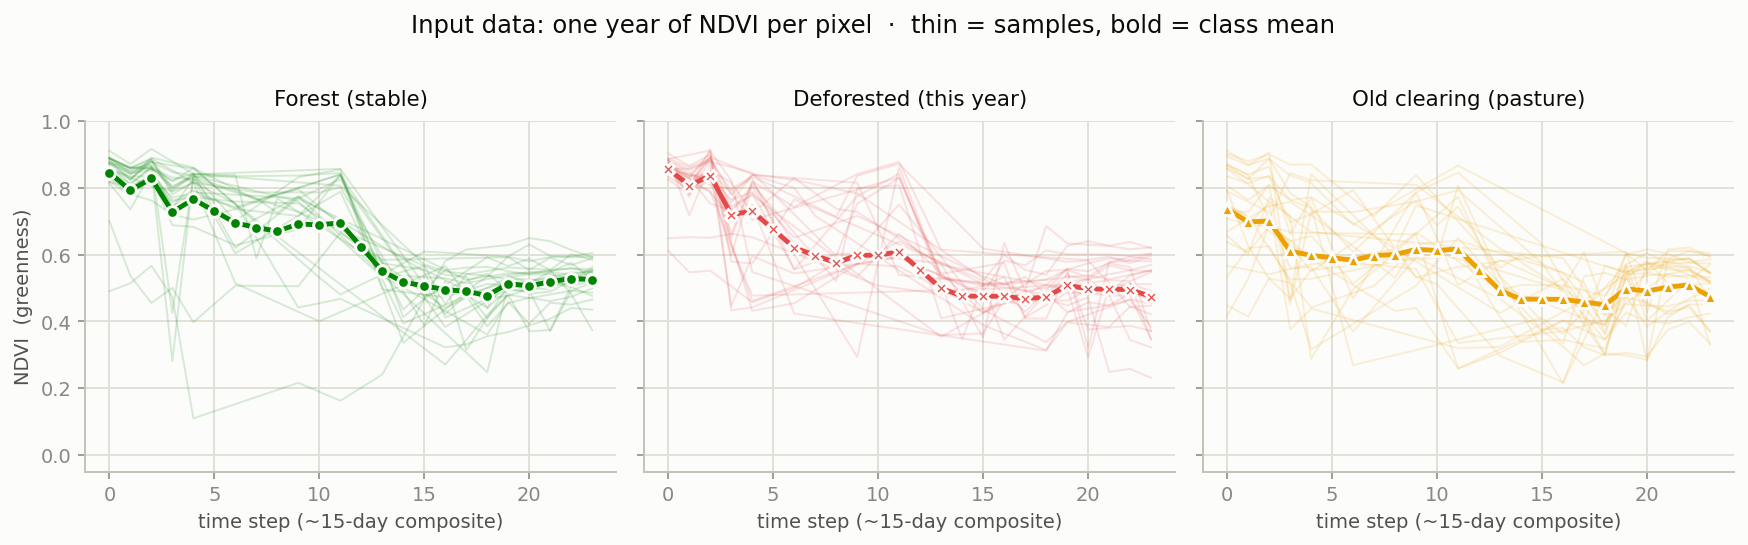
\includegraphics[width=0.96\textwidth]{fig_01_data_input.png}
  \begin{itemize}\small
    \item Thin lines = individual pixels; bold = class mean.
    \item \alert{Reality check:} even ``stable'' forest \emph{sags} to $\sim$0.5
          in the wet season — unavoidable residual cloud. Forest vs.\ deforested
          are \textbf{hard to separate with NDVI alone here}. Keep this in mind
          when we read the results.
  \end{itemize}
\end{frame}

\begin{frame}{Splitting train vs.\ test — \emph{spatially}}
  \begin{columns}[T]
    \begin{column}{0.55\textwidth}
      \begin{itemize}
        \item We hold out the \gtag{eastern 30\%} of the window (by longitude)
              as the test set.
        \item \textbf{Why not a random split?} Neighbouring pixels are
              correlated. A random split leaks near-identical pixels into both
              sets and \alert{inflates} the score.
        \item A spatial split is a harder, more \emph{honest} estimate of how the
              model does on \emph{new ground}.
      \end{itemize}
    \end{column}
    \begin{column}{0.45\textwidth}
      \centering
      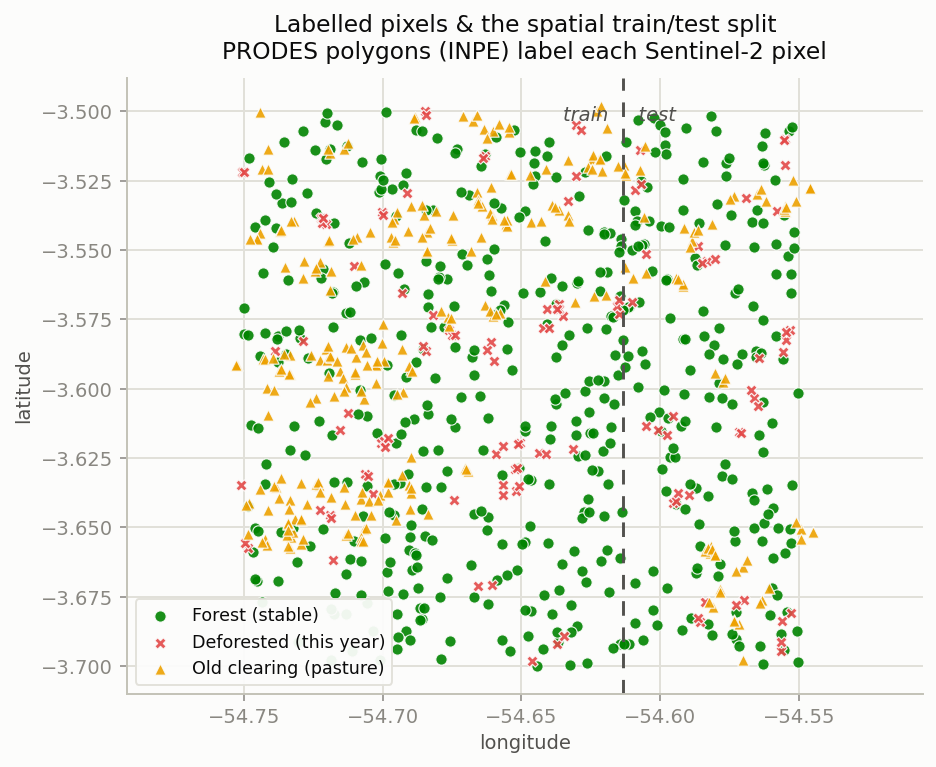
\includegraphics[width=\linewidth]{fig_02_labels.png}\\
      \src{Dashed line = the train/test boundary.}
    \end{column}
  \end{columns}
\end{frame}

% =========================================================================
\section{The technique}

\begin{frame}{Three models — and always a baseline first}
  \begin{block}{Methodology principle}
    Start simple. If a deep model can't beat a classical baseline, the added
    complexity isn't paying off.
  \end{block}
  \begin{columns}[T]
    \begin{column}{0.33\textwidth}
      \textbf{Baseline: Random Forest}
      \begin{itemize}\small
        \item The 24 NDVI values as 24 plain features.
        \item 200 trees, no temporal structure assumed.
        \item Close to what INPE used \emph{before} deep learning.
      \end{itemize}
    \end{column}
    \begin{column}{0.33\textwidth}
      \textbf{Deep model 1: 1D CNN}
      \begin{itemize}\small
        \item Convolutions slide \gtag{along time}, learning shapes like
              ``a mid-year drop''.
        \item $<$10k parameters; trains in minutes on CPU.
        \item Length-robust via global pooling.
      \end{itemize}
    \end{column}
    \begin{column}{0.33\textwidth}
      \textbf{Deep model 2: Transformer}
      \begin{itemize}\small
        \item \gtag{Self-attention}: every time step compares itself with
              every other.
        \item Needs a \emph{positional encoding} — attention is order-blind.
        \item Kept tiny ($\sim$10k params): 630 training samples punish
              capacity.
      \end{itemize}
    \end{column}
  \end{columns}
\end{frame}

\begin{frame}{The 1D-CNN architecture (\texttt{SITSCNN})}
  \centering
  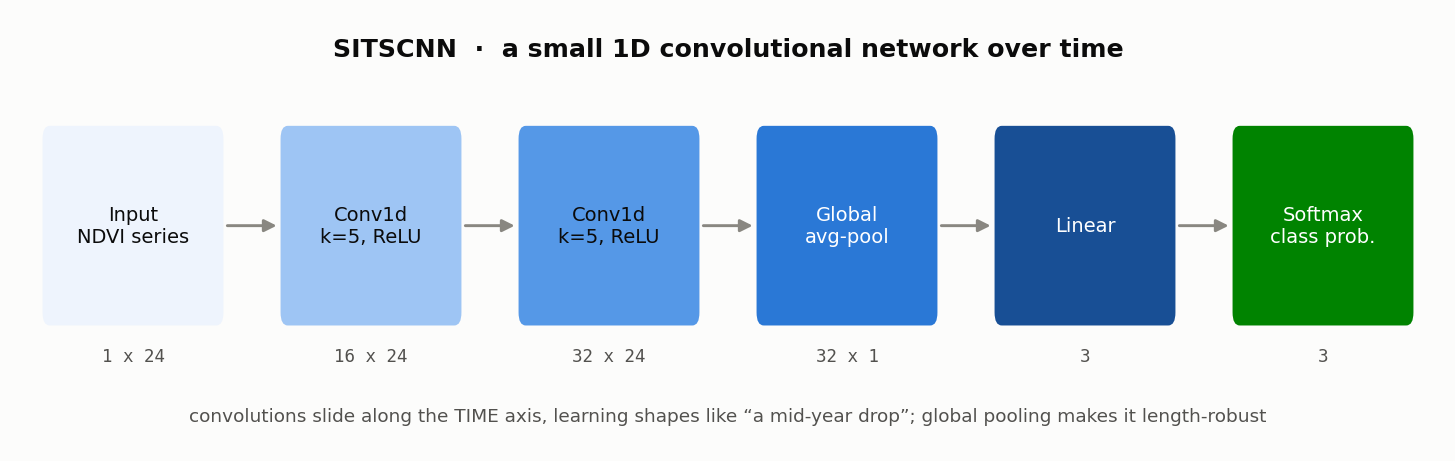
\includegraphics[width=0.98\textwidth]{fig_03_model.png}
  \begin{itemize}\small
    \item Two \texttt{Conv1d} layers (kernel 5) detect local temporal patterns;
          \textbf{global average pooling} summarises the whole year into 32
          numbers regardless of length; a linear head maps to 3 class scores.
    \item \gtag{Key idea:} the convolution finds ``a drop'' \emph{wherever} in
          the year it occurs — it is shift-invariant in time.
  \end{itemize}
\end{frame}

\begin{frame}{The transformer architecture (\texttt{SITSTransformer})}
  \centering
  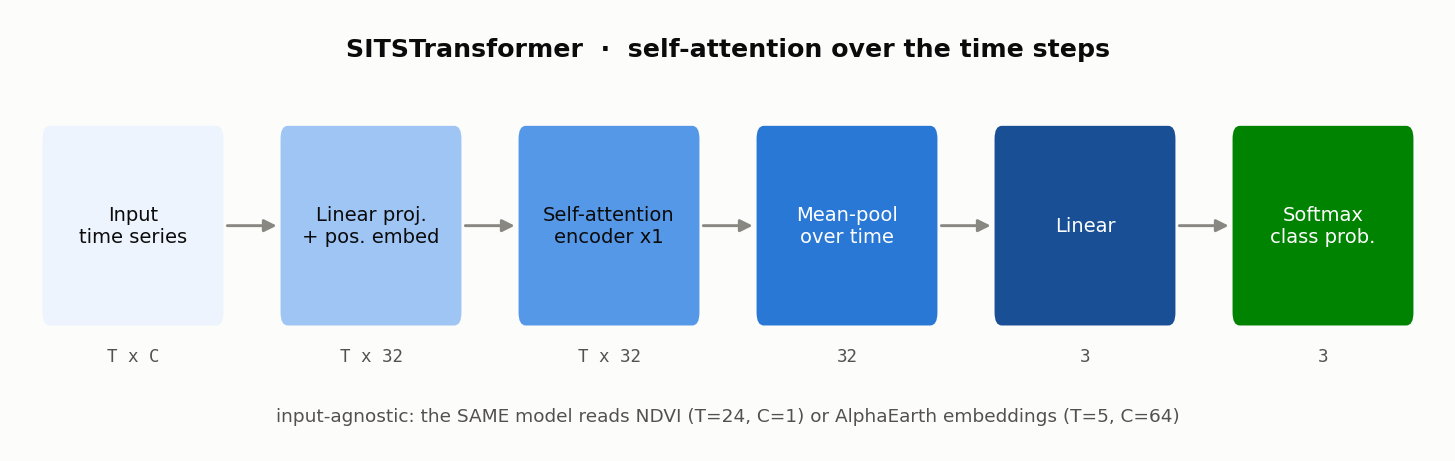
\includegraphics[width=0.98\textwidth]{fig_06_transformer.png}
  \begin{itemize}\small
    \item A linear layer lifts each time step to 32 dimensions; a
          \textbf{learned positional embedding} injects time order; one
          self-attention encoder layer lets steps exchange information;
          mean-pooling and a linear head give 3 class scores.
    \item \gtag{Input-agnostic by design:} it takes $(\text{batch}, T, C)$ for
          \emph{any} $T$ and $C$ — the \textbf{same class} reads the NDVI
          series ($24 \times 1$) and the AlphaEarth series ($5 \times 64$).
  \end{itemize}
\end{frame}

\begin{frame}{Training the network}
  \begin{columns}[T]
    \begin{column}{0.56\textwidth}
      \centering
      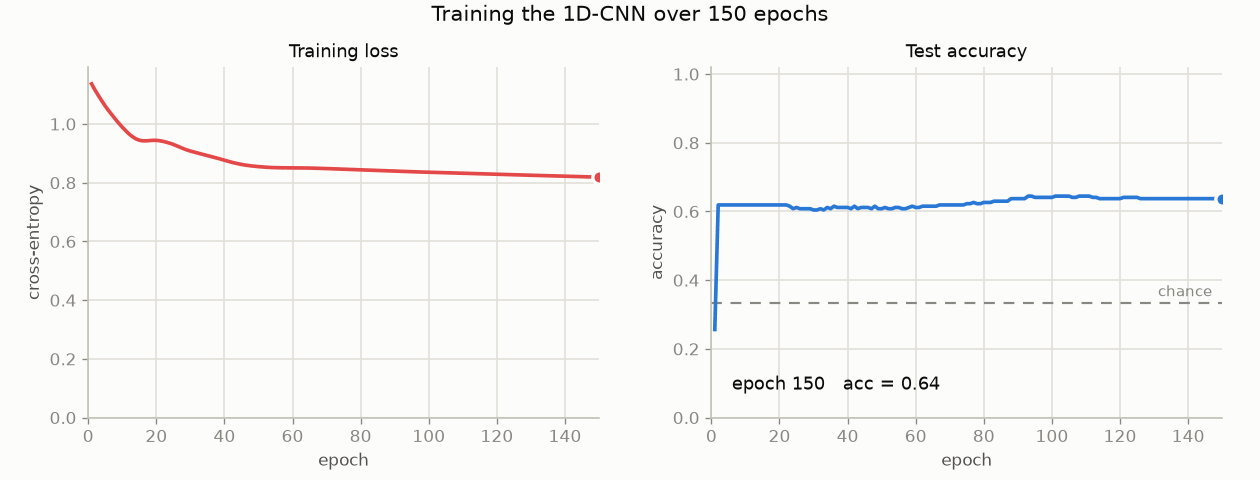
\includegraphics[width=\linewidth]{fig_03b_training.png}
    \end{column}
    \begin{column}{0.44\textwidth}
      \small
      \begin{itemize}
        \item Cross-entropy loss, Adam (lr $3\times10^{-3}$), 150 full-batch
              epochs.
        \item Loss falls, test accuracy plateaus around \textbf{0.64} — well
              above the 0.33 chance line, but \alert{watch what it's learning}.
      \end{itemize}
      \begin{exampleblock}{Best-practice: measure the cost}
        We wrap training in \textbf{CodeCarbon} to log energy \& CO$_2$.
        Negligible here — but imagine training over \emph{all} of Brazil,
        repeatedly.
      \end{exampleblock}
    \end{column}
  \end{columns}
\end{frame}

% =========================================================================
\section{Results \& interpretation}

\begin{frame}{Results — accuracy is not the whole story}
  \centering
  \begin{tabular}{@{}lccc@{}}
    \toprule
    \textbf{Model} & \textbf{Accuracy} & \textbf{Macro-F1} &
      \textbf{Deforested recall} \\
    \midrule
    \textcolor{accentblue}{Random Forest (baseline)} & 0.68 &
      \textbf{0.59} & \textbf{0.39} \\
    1D CNN & 0.64 & 0.41 & \alert{0.00} \\
    Transformer (NDVI) & \textbf{0.69} & 0.58 & 0.22 \\
    Transformer (AlphaEarth) & \multicolumn{3}{c}{\src{pending real
      embedding extraction — script in repo}} \\
    \bottomrule
  \end{tabular}
  \vspace{1em}
  \begin{itemize}
    \item The CNN's decent-looking accuracy hides a failure: it detects
          \alert{none} of the deforested class. \textbf{Accuracy alone lied.}
    \item The transformer does better — but the \gtag{simple baseline still
          finds the most actual deforestation}. Complexity must earn its place.
    \item \src{Spatial split; 635 train / 273 test pixels; 150 epochs each.}
  \end{itemize}
\end{frame}

\begin{frame}{Foundation features vs.\ hand-crafted NDVI}
  \begin{columns}[T]
    \begin{column}{0.52\textwidth}
      \centering
      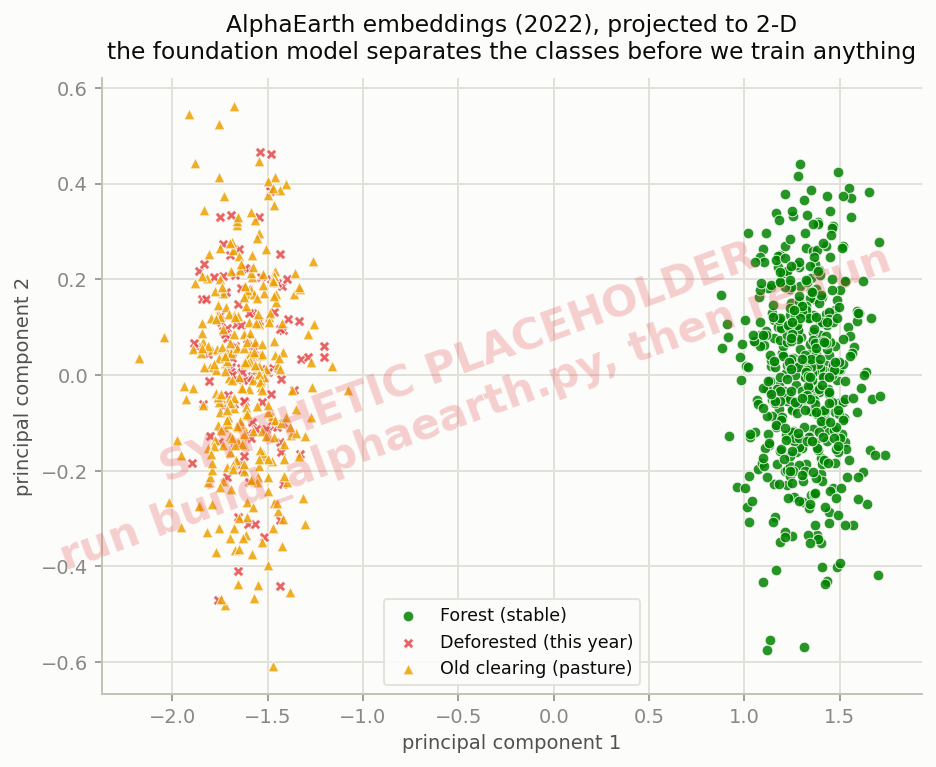
\includegraphics[width=\linewidth]{fig_08_alphaearth_pca.png}
    \end{column}
    \begin{column}{0.48\textwidth}
      \begin{itemize}\small
        \item A 2-D projection (PCA) of the 64-d AlphaEarth embeddings,
              \emph{before any training of ours}.
        \item If the foundation model has done its job, the classes already
              form \gtag{separable clusters} — our tiny transformer only has
              to draw the boundaries.
        \item The honest question of Section 9 in the notebook: do learned
              features beat a simple vegetation index \emph{on this task}?
      \end{itemize}
      \src{Figure regenerates from the real CSV once
        \texttt{build\_alphaearth.py} has been run.}
    \end{column}
  \end{columns}
\end{frame}

\begin{frame}{A leakage trap — post-event years}
  \begin{alertblock}{Annual embeddings can contain the answer}
    The label says ``cleared in 2022''. An AlphaEarth embedding for
    \textbf{2023 or 2024} summarises a year in which the land was
    \emph{already bare} — using it is like answering ``was this cleared in
    2022?'' while looking at a photo from 2024.
  \end{alertblock}
  \begin{itemize}
    \item Include the post-event years and \gtag{deforested recall jumps} —
          but the model has learned to \alert{read the answer off the input},
          not to detect a clearing.
    \item In production those ``future'' features \textbf{do not exist} at
          prediction time. The notebook defaults to years $\leq$ 2022 and
          turns the leak into an exercise.
    \item General lesson: with temporal data, always ask —
          \emph{would this feature have existed when the prediction was
          needed?}
  \end{itemize}
\end{frame}

\begin{frame}{Where the CNN goes wrong — the confusion matrix}
  \begin{columns}[T]
    \begin{column}{0.5\textwidth}
      \centering
      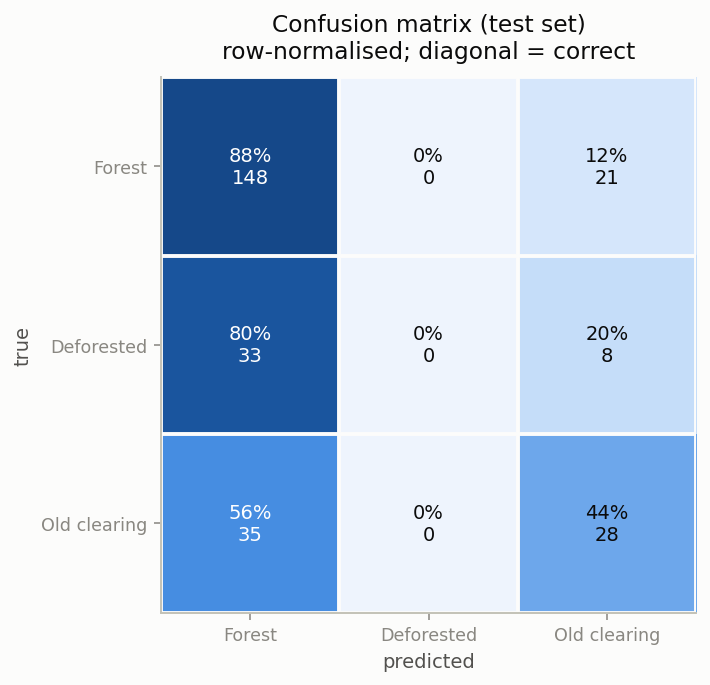
\includegraphics[width=0.92\linewidth]{fig_04_confusion.png}
    \end{column}
    \begin{column}{0.5\textwidth}
      \begin{itemize}
        \item The \alert{``deforested'' column is empty} — the model never
              predicts it.
        \item It defaults to the majority ``forest'' class, because
              \begin{itemize}\small
                \item deforested is the \textbf{minority} (116 of 908), and
                \item its NDVI shape \textbf{overlaps} forest in this cloudy
                      window.
              \end{itemize}
        \item This is \gtag{class imbalance} + \gtag{weak signal} — the two
              failure modes the tutorial is built to expose.
      \end{itemize}
    \end{column}
  \end{columns}
\end{frame}

\begin{frame}{Predictions across the held-out region}
  \begin{columns}[T]
    \begin{column}{0.55\textwidth}
      \centering
      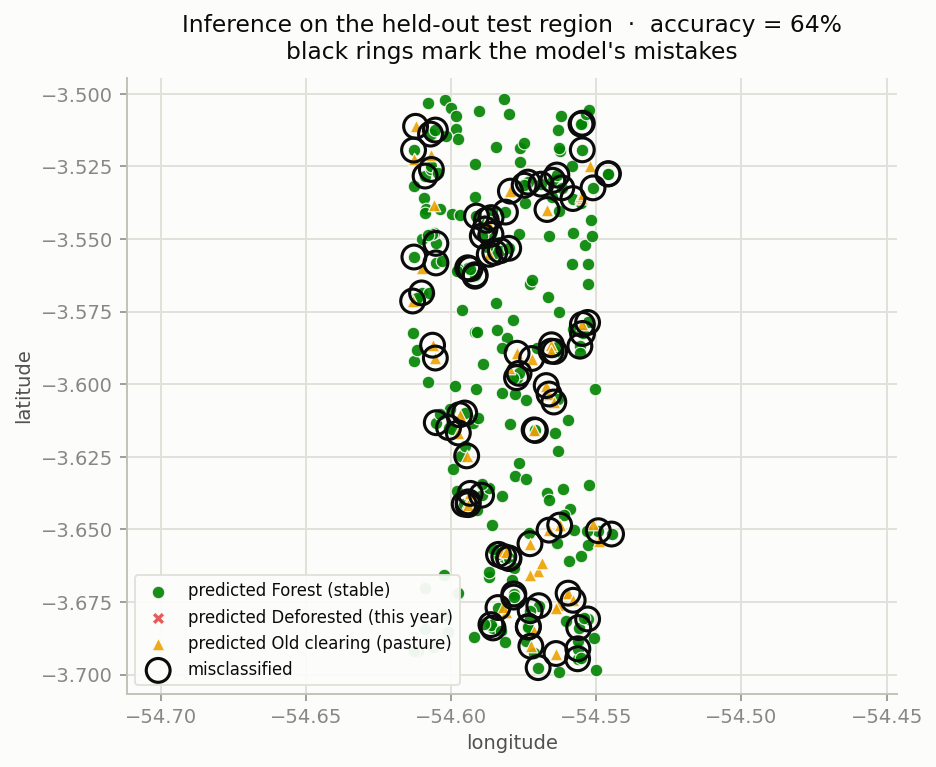
\includegraphics[width=\linewidth]{fig_05_inference_map.png}
    \end{column}
    \begin{column}{0.45\textwidth}
      \begin{itemize}
        \item Each point coloured by the model's \emph{prediction}; black rings
              mark mistakes.
        \item Errors are \alert{not random} — they cluster where clearings are,
              exactly the places we most need to get right.
        \item A map like this is how an analyst would \emph{visually audit} a
              model before trusting it.
      \end{itemize}
    \end{column}
  \end{columns}
\end{frame}

\begin{frame}{Reading the results — the real lesson}
  \begin{block}{What a good analyst concludes here}
    \begin{enumerate}
      \item \textbf{Never trust accuracy alone} on imbalanced data — read
            per-class recall and the confusion matrix.
      \item \textbf{Baselines matter} — the RF beat the CNN; complexity must
            earn its place.
      \item \textbf{The data limits the model} — NDVI alone, in a cloudy
            window, can't cleanly separate forest from fresh clearing.
    \end{enumerate}
  \end{block}
  \gtag{Fixes to try} (interactive): class weighting / resampling, more
  bands \& indices (SWIR, NBR, radar), a longer clean time window, or a spatial
  (image) model instead of a per-pixel one.
\end{frame}

% =========================================================================
\section{Limitations \& responsible use}

\begin{frame}{Limitations — what this cannot tell us}
  \begin{itemize}
    \item \textbf{One region, one year, one sensor} $\Rightarrow$ does
          \alert{not generalise}. A model tuned here will fail elsewhere.
    \item \textbf{Balanced classes} misrepresent the true rarity of
          deforestation; real performance would look worse.
    \item \textbf{NDVI-only} is blind to degradation, selective logging, and
          some fire.
    \item \textbf{Interpolated cloud gaps} hide genuine data messiness.
    \item \textbf{PRODES labels} are annual and clear-cut focused — the ceiling
          on what we can learn.
  \end{itemize}
\end{frame}

\begin{frame}{Responsible use — who is affected if we're wrong}
  \begin{columns}[T]
    \begin{column}{0.5\textwidth}
      \begin{alertblock}{Consequences of error}
        \begin{itemize}\small
          \item A \emph{false} ``deforested'' can wrongly flag a landholder
                (inspection, credit denial).
          \item A \emph{missed} clearing lets destruction go undetected.
        \end{itemize}
      \end{alertblock}
    \end{column}
    \begin{column}{0.5\textwidth}
      \textbf{Before any real use, you need:}
      \begin{itemize}\small
        \item independent validation vs.\ high-res imagery,
        \item expert review of alerts,
        \item transparency about accuracy \& uncertainty,
        \item governance over who acts and how errors are appealed.
      \end{itemize}
      \src{The kind of safeguards INPE builds around PRODES / DETER.}
    \end{column}
  \end{columns}
  \vspace{0.3em}
  \centering
  \textbf{This is a teaching model — \alert{not} for enforcement, fines, trade
  compliance, or operational mapping.}
\end{frame}

% =========================================================================
\section{Wrap-up}

\begin{frame}{Summary}
  \begin{itemize}
    \item We framed deforestation detection as \gtag{time-series
          classification} of NDVI, built from \textbf{Sentinel-2} imagery and
          \textbf{PRODES} labels over a real Amazon frontier.
    \item We built a reproducible dataset and compared a \textbf{Random
          Forest} baseline, a \textbf{1D CNN} and a \textbf{time series
          Transformer}, evaluated with a spatial split.
    \item The honest result: \alert{modest accuracy, and deep models that
          struggle with the minority class} — a lesson in imbalance, weak
          signals, and reading metrics critically.
    \item \textbf{AlphaEarth} embeddings turn the task into a multi-year
          sequence the \emph{same} transformer can read — and teach a second
          lesson: \alert{temporal label leakage}.
    \item Responsible-use thinking runs \emph{throughout}, not as an afterthought.
  \end{itemize}
  \vspace{0.5em}
  \centering
  \gtag{From concept $\to$ data $\to$ model $\to$ evaluation $\to$ judgement.}
\end{frame}

\begin{frame}[standout]
  Questions?\\[0.4em]
  \small\normalfont Run it yourself: the notebook, dataset builder, and these
  figures are all in the tutorial repository.
\end{frame}

\appendix
\begin{frame}[allowframebreaks]{Sources \& further reading}
  \footnotesize
  \begin{itemize}
    \item IPCC AR6 WGIII, Ch.~7 (AFOLU); Ometto et al., 2022.
    \item INPE PRODES \& DETER — \texttt{terrabrasilis.dpi.inpe.br}.
    \item ESA Copernicus Sentinel-2; Microsoft Planetary Computer STAC.
    \item Gebru et al., ``Datasheets for Datasets'', 2021 (see \texttt{DATASHEET.md}).
    \item Mitchell et al., ``Model Cards for Model Reporting'', 2019
          (see \texttt{MODEL\_CARD.md}).
    \item EU Deforestation Regulation (EU) 2023/1115.
    \item Vaswani et al., ``Attention Is All You Need'', 2017.
    \item Sainte Fare Garnot \& Landrieu, ``Lightweight Temporal Self-Attention
          for Classifying Satellite Image Time Series'', 2020.
    \item Brown et al., ``AlphaEarth Foundations'', 2025; Satellite Embedding
          dataset in Google Earth Engine
          (\texttt{GOOGLE/SATELLITE\_EMBEDDING/V1\_ANNUAL}).
  \end{itemize}
\end{frame}

\end{document}
